% 三维投影
% 立体几何|投影|透视|画图

% 参考 https://en.wikipedia.org/wiki/3D_projection

当我们在平面上画三维物体时, 我们需要某种投影算法把物体上的每个点对应到平面上的一点. 以下介绍两种常用的方法, 一种是\textbf{平行投影(parallel projection)}, 另一种是\textbf{透视投影(perspective projection)}.

% 首先来比较两个图(图未完成: 左图是长方体的平行投影, 右图是长方体的透视投影)
% 参考 https://construct3.ideas.aha.io/ideas/C3-I-754

\subsection{平行投影}
顾名思义, 平行投影是指在空间中指定一个方向(如图未完成), 将三维物体上的每一点沿着该方向投影到与该方向垂直的平面上. 工程制图中的正视图, 侧视图等都属于平行投影. 这种投影的特点是, 空间中的任意两条平行线的投影仍然是平行线.

\subsection{透视投影}
当人眼或相机观察一个三维物体时, 使用的是透视投影.

(用一张图介绍原理)

我们在平面后方取一个固定点 $F$ 称为\textbf{焦点}, 要把物体上任意一点 $P$ 投影到平面上, 先作直线 $PF$, 该直线与平面的交点 $P'$ 就是投影后的点. 我们在平面上建立直角坐标系, 把平面上离焦点最近的点定义为平面坐标的原点.

为什么透视投影要这样定义? 我们先思考一种非常简单的相机, 即小孔成像相机. 根据光的直线传播, 物体上的某点发出的(或反射的)光线只有经过小孔才能投影到孔后面的平面. 如果按照这个模型, 我们在计算透视投影时应该把焦点定义在屏幕之前, 然而这么做有一个缺点就是投影后平面上的像是倒像. 所以为了方便起见, 我们保持焦点不变, 但是把屏幕平移到焦点之前(焦距也不变), 容易看出这样做的唯一改变就是把倒像变为正像, 即点 $P'$ 的两个平面坐标分别取相反数. % (未完成)需要一张图比较焦点在前和焦点在后

如果我们将相机上的小孔改为焦距为 $f$ 的小凸透镜, 并假设物距远大于焦距, 那么根据成像公式, 凸透镜和平面(即底片)的距离就是焦距 $f$. 根据凸透镜成像原理, 物体一点在底片上的像仍然会过凸透镜的中点% 图未完成
, 所以使用凸透镜的相机和使用小孔成像的相机得到的投影是相同的. 至于人眼, 人眼成像的原理和相机基本一致, 虽然视网膜并不是一个平面, 得到的成像是扭曲的, 但大脑在处理图象是会自动纠正这种扭曲(例如我们看到的直线仍然是直的).

\subsection{计算方法}
(未完成: 另外开一篇文章分享平行投影和透视投影的 Matlab 代码)

\subsection{3D 艺术画}
(未完成, 用一张示意图说明如何用一张正常的图生成 3D 艺术画)
\begin{figure}[ht]
\centering
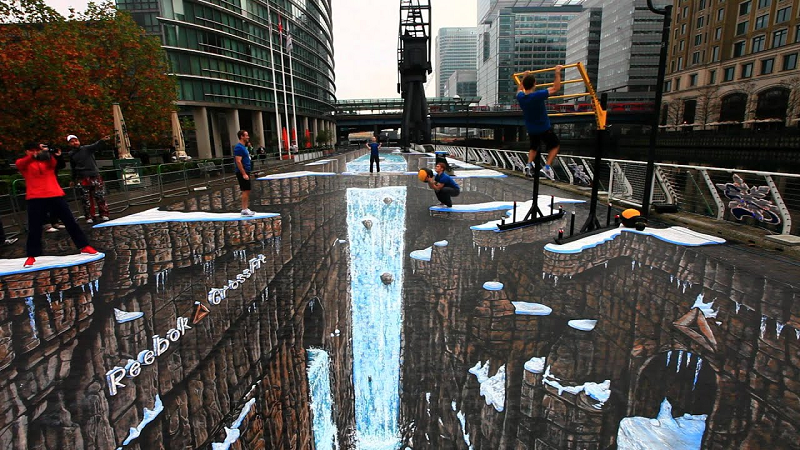
\includegraphics[width=10cm]{./figures/proj3D_1.png}
\caption{2011 年最大的 3D 艺术画, 画于伦敦街头, 获吉尼斯纪录} \label{proj3D_fig1}
\end{figure}

\begin{figure}[ht]
\centering
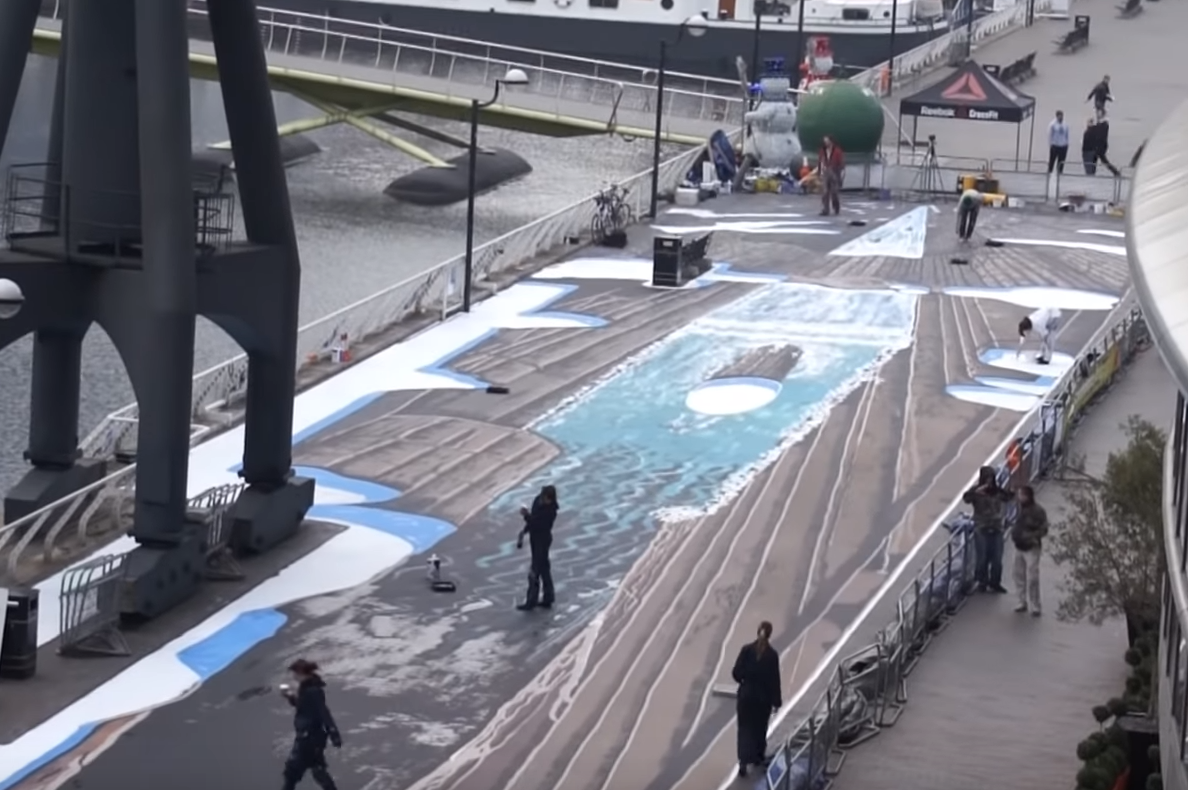
\includegraphics[width=10cm]{./figures/proj3D_2.png}
\caption{从不同角度看 3D 艺术画(\autoref{proj3D_fig1} 由该图中右上角相机拍摄)} \label{proj3D_fig2}
\end{figure}

(未完成: 另外开一篇文章分享代码)
